% Experiments (condensed for the two-column paper, step 4). Numbers from paper/tables/* (scripts/build_paper.py),
% results/stats/e5_convergence.*, results/stats/e7_montecarlo.*; supplement items cited with \Sref.
\section{Experiments}
\label{sec:experiments}

\subsection{Setup}
\label{sec:setup}
\emph{Suite A} reproduces the instance sizes of \citet{jin2026imoeadqn}: 3, 6 or 10 edge servers, 100, 300 or 500 tasks,
and 20--250 devices that each submit a layered random DAG. Workloads are 1--5 Gcycles and data 500--3000 KB as in Jin et
al., used as given and multiplied by 20; this gives 12 test instances. 36 further instances generated with other seeds
were used only to set the method's parameters. \emph{Suite B} takes five scientific workflow families from WfCommons
\citep{coleman2022wfcommons} (Cybershake, Epigenomics, Inspiral, Montage, Sipht) with 100, 400 and 1000 tasks in Jin et
al.'s small scenario (3 edge servers, 6 devices), with sizes mapped into Jin et al.'s ranges, interval half-widths of
5--30\% and data multiplied by 1, 20 or 100: 45 instances. Table~\Sref{tab:params} of the supplementary material lists all
parameters.

We compare \ours{} with four interval evolutionary algorithms, IMOEA/D with the original settings reported by
\citet{cui2024imeaied}, IMOEA/D-AWN \citep{jin2023imoeadawn}, IMEA-IED \citep{cui2024imeaied} and IP-MOEA
\citep{limbourg2005ipmoea}; with NSGA-II \citep{deb2002nsga2} on interval midpoints or by interval dominance and NSGA-III
\citep{deb2014nsga3}; and with IMOEA-DQN \citep{jin2026imoeadqn} and its backbone run with the fixed action
$(5/6, 1/6, 0)$ (the \emph{Jin backbone}), which isolates the effect of Rank C and the mating. All methods share the
encoding, operators, evaluator, $N = 105$ and the budget of $N(G_{\max}+1)$ evaluations with $G_{\max} = 1000$.
IGD is measured on interval midpoints against the non-dominated union of all final fronts, and HV is the mean of the
lower- and upper-bound hypervolumes (reference 1.1), both after normalising each instance once over all methods.
\ours{}, IMOEA/D and the Jin backbone were run 30 times, the others 10 times; methods are compared per instance by the
Wilcoxon rank-sum test with Holm's correction \citep{holm1979} and over instances by Friedman ranks \citep{demsar2006}.

% generated by scripts/build_paper.py; do not edit by hand
\begin{table*}[!htbp]
\centering
\footnotesize
\caption{Results on both suites: mean IGD ($\times10^{-2}$) and HV over instances, the number of instances on which each method is significantly better / worse / not different from \ours{} (Wilcoxon rank-sum, Holm-corrected, $\alpha = 0.05$), and the mean Friedman rank by IGD (Nemenyi critical difference 3.91 on Suite A, 2.02 on Suite B). Per-instance results are in the supplementary material.}
\label{tab:summary}
\setlength{\tabcolsep}{3pt}
\begin{tabular}{lcccccccccc}
\toprule
& \multicolumn{5}{c}{Suite A (12 instances)} & \multicolumn{5}{c}{Suite B (45 instances)} \\
\cmidrule(lr){2-6}\cmidrule(lr){7-11}
Method & IGD & HV & IGD $+/-/\approx$ & HV $+/-/\approx$ & Rank & IGD & HV & IGD $+/-/\approx$ & HV $+/-/\approx$ & Rank \\
\midrule
\ours{} & \textbf{1.22} & \textbf{0.819} & -- & -- & 1.00 & \textbf{1.86} & \textbf{0.949} & -- & -- & 1.29 \\
IMOEA/D & 3.19 & 0.797 & 0/12/0 & 0/12/0 & 2.83 & 2.57 & 0.935 & 1/43/1 & 2/42/1 & 2.69 \\
IMOEA/D-AWN & 2.91 & 0.797 & 0/12/0 & 0/12/0 & 2.42 & 4.44 & 0.915 & 0/43/2 & 0/44/1 & 3.29 \\
IMEA-IED & 12.40 & 0.691 & 0/12/0 & 0/12/0 & 7.17 & 13.34 & 0.828 & 0/45/0 & 0/45/0 & 7.73 \\
IP-MOEA & 14.71 & 0.658 & 0/12/0 & 0/12/0 & 8.50 & 12.24 & 0.822 & 0/45/0 & 0/45/0 & 6.98 \\
NSGA-II (mid) & 4.84 & 0.770 & 0/12/0 & 0/12/0 & 4.50 & 6.51 & 0.882 & 4/40/1 & 0/44/1 & 3.82 \\
NSGA-II (int) & 4.80 & 0.771 & 0/12/0 & 0/12/0 & 4.25 & 6.57 & 0.882 & 5/40/0 & 0/44/1 & 4.09 \\
NSGA-III & 13.61 & 0.690 & 0/12/0 & 0/12/0 & 7.75 & 15.42 & 0.822 & 0/45/0 & 0/45/0 & 8.40 \\
Jin backbone & 11.66 & 0.635 & 0/12/0 & 0/12/0 & 6.67 & 11.64 & 0.805 & 0/45/0 & 0/45/0 & 6.78 \\
IMOEA-DQN & 25.43 & 0.605 & 0/12/0 & 0/12/0 & 9.92 & 22.94 & 0.736 & 0/45/0 & 0/45/0 & 9.93 \\
\bottomrule
\end{tabular}
\end{table*}


\subsection{Comparison with the baselines}
\label{sec:results}
Table~\ref{tab:summary} summarises both suites. On Suite A, \ours{} has the best IGD and HV on all 12 instances, with a
mean IGD 62\% below IMOEA/D's and Friedman rank 1.00. On Suite B it is better than IMOEA/D on 43 of 45 instances in IGD
and 42 in HV; IMEA-IED, IP-MOEA, NSGA-III, the Jin backbone and IMOEA-DQN lose on every instance, and IMOEA/D-AWN is never
better. NSGA-II reaches a lower IGD on 4--5 instances, all 100-task workflows with data $\times 1$, and never a higher HV.
The Jin backbone, with the same fixed action, has a six times higher IGD (0.116), and its gap grows with the DAG, as
Section~\ref{sec:stall} predicts. The intervals of \ours{} are slightly wider than IMOEA/D's (Suite B imprecision 60.9
against 57.8; Table~\Sref{tab:suiteb_imprecision}); the methods with narrower intervals keep much smaller fronts.
Per-instance results are in Tables~\Sref{tab:suitea_igd}--\Sref{tab:suiteb_hv_jin} and list-scheduling heuristics,
16--33 times worse in IGD, in Table~\Sref{tab:heuristics}.

The comparison with IMOEA/D depends on the normalisation at one size only. Repeating it with four different method
pools defining the normalisation and the reference front (Table~\Sref{tab:robustness}) leaves every verdict on Suite A
and up to 400 tasks, and every HV verdict, unchanged; at 1000 tasks, however, IMOEA/D has the lower IGD on 6--9 of 15
instances when only the strong methods form the pool. We therefore read the 1000-task results on HV, where \ours{} is
better on 12 of 15.

\subsection{Convergence and ablation}
\label{sec:convergence}
\label{sec:ablation}
Fig.~\ref{fig:e5_convergence} shows that \ours{} pulls ahead of every method by generation 100 on medium-250 and ends
with a third of IMOEA/D's IGD (0.012 against 0.035). On montage-400, IMOEA/D converges faster at first and \ours{}
overtakes it at about generation 350. On the 1000-task workflows the two are close throughout, \ours{} ends slightly
ahead, and both curves are still falling at generation 1000. IMOEA-DQN starts worse than the initial population because
its early actions concentrate the search in one region.

\begin{figure*}[pos=tbp]
\centering
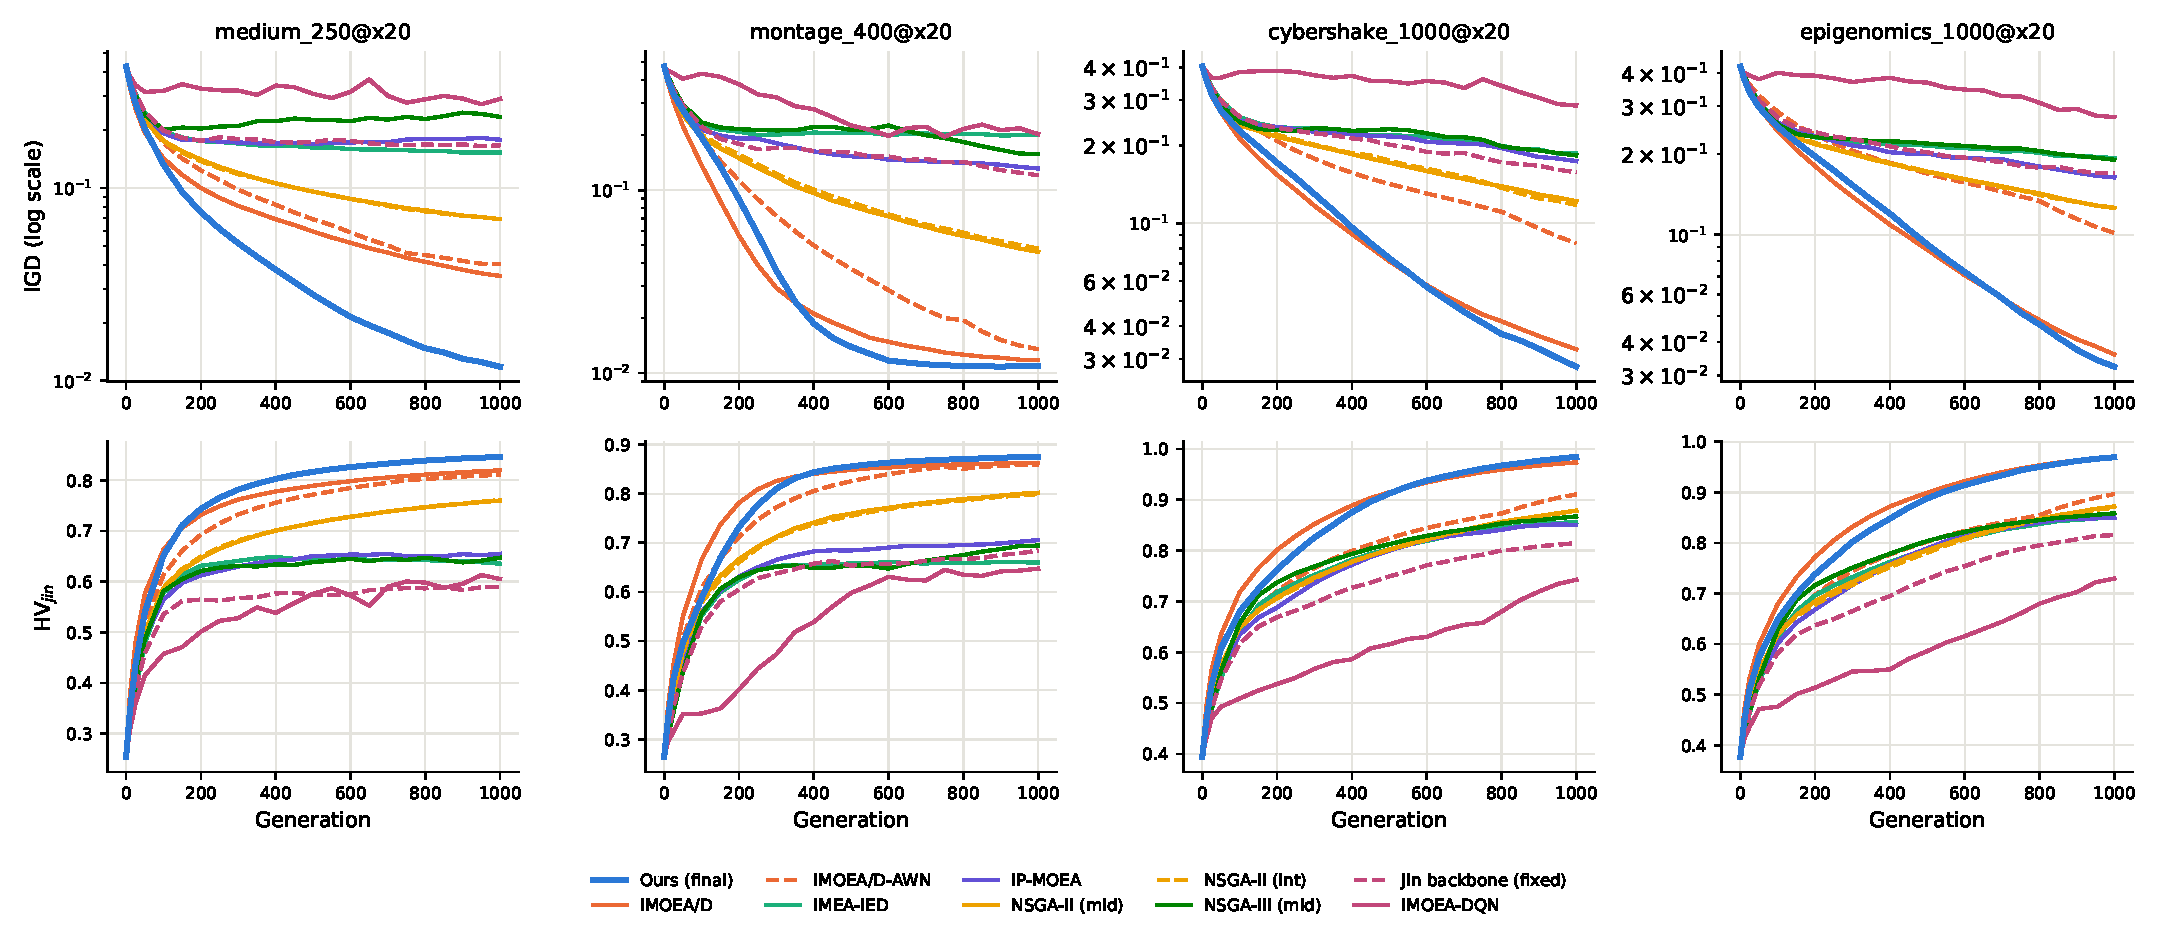
\includegraphics[width=\textwidth]{figures/e5_convergence.pdf}
\caption{Mean IGD (top, log scale) and HV (bottom) against the generation, 10 runs per method, on one Suite A and three
Suite B instances (data $\times 20$).}
\label{fig:e5_convergence}
\end{figure*}

Table~\ref{tab:ablation} builds \ours{} from the Jin backbone. The Tchebycheff Rank C halves the IGD, the ICD tie-break
lowers it further, and neighbourhood mating brings it from 0.048 to 0.0135; together the rank and the mating are 3.5
times better than either alone. Smaller, always-local neighbourhoods and $N$ weight vectors are best, and even the
untuned action $(1, 0, 0)$ beats IMOEA/D (0.0175 against 0.0314).

% generated by scripts/build_paper.py; do not edit by hand
\begin{table}[!htbp]
\centering
\footnotesize
\caption{Ablation on the 12 Suite A instances (10 runs; IGD $\times10^{-2}$, means over instances). $+/-/\approx$: instances where the variant is significantly better / worse / not different from the reference in the group heading (Wilcoxon rank-sum, $\alpha = 0.05$).}
\label{tab:ablation}
\setlength{\tabcolsep}{3pt}
\begin{tabular}{lccc}
\toprule
Variant & IGD & HV & IGD $+/-/\approx$ \\
\midrule
\multicolumn{4}{l}{\textit{Build-up (vs \ours{})}} \\
\quad Jin et al.\ backbone & 11.86 & 0.630 & 0/12/0 \\
\quad + Tchebycheff Rank C & 5.76 & 0.760 & 0/12/0 \\
\quad + ICD tie-break & 4.80 & 0.769 & 0/12/0 \\
\quad + mating, $T{=}20$, $p{=}0.9$ & 1.35 & 0.806 & 0/9/3 \\
\quad \ours{} ($T{=}10$, $p{=}1$) & 1.02 & 0.814 & -- \\
\midrule
\multicolumn{4}{l}{\textit{Leave one out (vs $T{=}20$)}} \\
\quad without Tchebycheff & 6.83 & 0.664 & 0/12/0 \\
\quad without ICD tie-break & 1.63 & 0.801 & 0/8/4 \\
\quad without mating & 4.80 & 0.769 & 0/12/0 \\
\midrule
\multicolumn{4}{l}{\textit{Parameters (vs $T{=}20$)}} \\
\quad $T = 10$ & 1.07 & 0.812 & 9/0/3 \\
\quad $T = 40$ & 2.38 & 0.792 & 0/12/0 \\
\quad $p_{local} = 0.5$ & 2.01 & 0.796 & 0/11/1 \\
\quad $N/2$ weight vectors & 1.80 & 0.803 & 0/12/0 \\
\quad $2N$ weight vectors & 1.90 & 0.792 & 0/11/1 \\
\quad action $(1, 0, 0)$ & 1.75 & 0.801 & 0/7/5 \\
\bottomrule
\end{tabular}
\end{table}


\subsection{Sensitivity, scalability and realised values}
\label{sec:sensitivity}
\label{sec:montecarlo}
\label{sec:runtime}
Table~\ref{tab:sensitivity} changes one setting at a time. \ours{} keeps the lower mean IGD in every case; IMOEA/D comes
close only when the energy of all three tiers is counted and, on HV, with doubled interval widths. At 2000 tasks
\ours{} has the higher HV on 13 of 15 instances while IGD is level (5 wins, 6 losses, 4 ties for IMOEA/D): IMOEA/D
reaches cheaper solutions at the cost end of the front, although \ours{}'s front dominates 64--79\% of IMOEA/D's where
they overlap.

To check the intervals against reality, we evaluated every final front under 200 crisp scenarios drawn uniformly from
the input intervals. Every realised objective vector lay inside its predicted interval, and the methods rank the same on
realised as on interval IGD (Kendall $\tau$ 0.91--1.00; Table~\Sref{tab:montecarlo}). \ours{} needs 29--62\,s per run,
about as long as IMOEA/D and less than IMOEA/D-AWN and IMEA-IED (Table~\Sref{tab:timing}).

% generated by scripts/build_paper.py; do not edit by hand
\begin{table}[!htbp]
\centering
\footnotesize
\caption{Sensitivity on the five 400-task workflows (data $\times 20$, 10 runs), one setting changed at a time, and scalability to 2000 tasks. Last two columns: instances where IMOEA/D is significantly better / worse / not different from \ours{} (Wilcoxon rank-sum, Holm, $\alpha = 0.05$). NSGA-II and the Jin backbone are worse on every instance in every setting (Table~\Sref{tab:sensitivity} of the supplementary material).}
\label{tab:sensitivity}
\setlength{\tabcolsep}{3pt}
\begin{tabular}{lcccc}
\toprule
& \multicolumn{2}{c}{IGD ($\times10^{-2}$)} & \multicolumn{2}{c}{IMOEA/D $+/-/\approx$} \\
\cmidrule(lr){2-3}\cmidrule(lr){4-5}
Setting & Ours & IMOEA/D & IGD & HV \\
\midrule
Base case & \textbf{0.82} & 1.21 & 0/5/0 & 0/5/0 \\
All-tier energy & \textbf{1.00} & 1.08 & 3/1/1 & 4/0/1 \\
Widths $\times 0.5$ & \textbf{0.94} & 1.78 & 0/5/0 & 0/5/0 \\
Widths $\times 2$ & \textbf{0.73} & 0.89 & 0/4/1 & 2/1/2 \\
Bandwidth $\times 0.5$ & \textbf{1.18} & 1.60 & 0/5/0 & 0/5/0 \\
Bandwidth $\times 2$ & \textbf{0.63} & 1.00 & 0/5/0 & 0/5/0 \\
1 edge server & \textbf{0.93} & 1.12 & 0/4/1 & 0/4/1 \\
6 edge servers & \textbf{1.08} & 1.70 & 0/4/1 & 0/5/0 \\
Edge queueing & \textbf{0.83} & 1.06 & 0/5/0 & 0/4/1 \\
\midrule
2000 tasks & 6.99 & \textbf{6.92} & 5/6/4 & 0/13/2 \\
\bottomrule
\end{tabular}
\end{table}


\subsection{Learned control of the selection weights}
\label{sec:learned}
IMOEA-DQN's central idea is to learn $(\alpha, \beta, \gamma)$ during the run. We tested three DQN designs on our
backbone, with and without a graph-attention encoder of the DAG \citep{velickovic2018gat}: Jin et al.'s per-generation
decisions with a population-indicator reward, one decision per 50 generations with a hypervolume reward, and one per 25
generations among the 10 actions with $\alpha \ge 1/2$. None beats the fixed action (Table~\ref{tab:learners}): the best
reaches an IGD of 0.0196 against 0.0143, close to a random choice among the same actions (0.0251), and the graph encoder
does not help consistently (Table~\Sref{tab:gat}). Fig.~\ref{fig:reward_audit} shows why. The summed reward ranks the
actions roughly like IGD (Spearman 0.90--0.92), but after generation 100 the reward of a single step is mostly noise:
the spread between actions is 0.02--0.08 of its standard deviation. With the best fixed action already within about
10\% of the best action on each instance, there is little for an adaptive schedule to gain and too little signal to
find it.

% generated by scripts/build_paper.py; do not edit by hand
\begin{table}[!htbp]
\centering
\footnotesize
\caption{Learned against fixed control of the selection weights on four Suite A instances (4 runs; IGD $\times10^{-2}$). All rows above \ours{} use the Tchebycheff backbone with $T = 20$, $p_{local} = 0.9$. $+/-/\approx$: instances where the row is significantly better / worse / not different from the fixed action $(5/6, 1/6, 0)$ (Wilcoxon rank-sum, $\alpha = 0.05$).}
\label{tab:learners}
\setlength{\tabcolsep}{3pt}
\begin{tabular}{lccc}
\toprule
Control of $(\alpha, \beta, \gamma)$ & IGD & HV & IGD $+/-/\approx$ \\
\midrule
\multicolumn{4}{l}{\textit{Fixed or random action}} \\
\quad Fixed $(5/6, 1/6, 0)$ & 1.43 & 0.784 & -- \\
\quad Fixed $(1, 0, 0)$ & 1.77 & 0.778 & 0/1/3 \\
\quad Random, $\alpha \ge 1/2$ & 2.51 & 0.751 & 0/4/0 \\
\midrule
\multicolumn{4}{l}{\textit{DQN control (interval, reward, actions)}} \\
\quad Every gen., PIBI, GAT & 3.67 & 0.759 & 0/4/0 \\
\quad Every gen., PIBI & 3.22 & 0.760 & 0/4/0 \\
\quad Every 50 gen., HV, GAT & 7.31 & 0.720 & 0/4/0 \\
\quad Every 50 gen., HV & 5.41 & 0.739 & 0/4/0 \\
\quad Every 25 gen., 10 act., GAT & 2.23 & 0.774 & 0/3/1 \\
\quad Every 25 gen., 10 act. & 1.96 & 0.778 & 0/2/2 \\
\midrule
\multicolumn{4}{l}{\textit{For comparison}} \\
\quad \ours{} & 1.21 & 0.792 & 3/0/1 \\
\quad IMOEA-DQN & 23.88 & 0.583 & 0/4/0 \\
\quad IMOEA/D & 2.92 & 0.770 & 0/4/0 \\
\bottomrule
\end{tabular}
\end{table}


\begin{figure*}[pos=tbp]
\centering
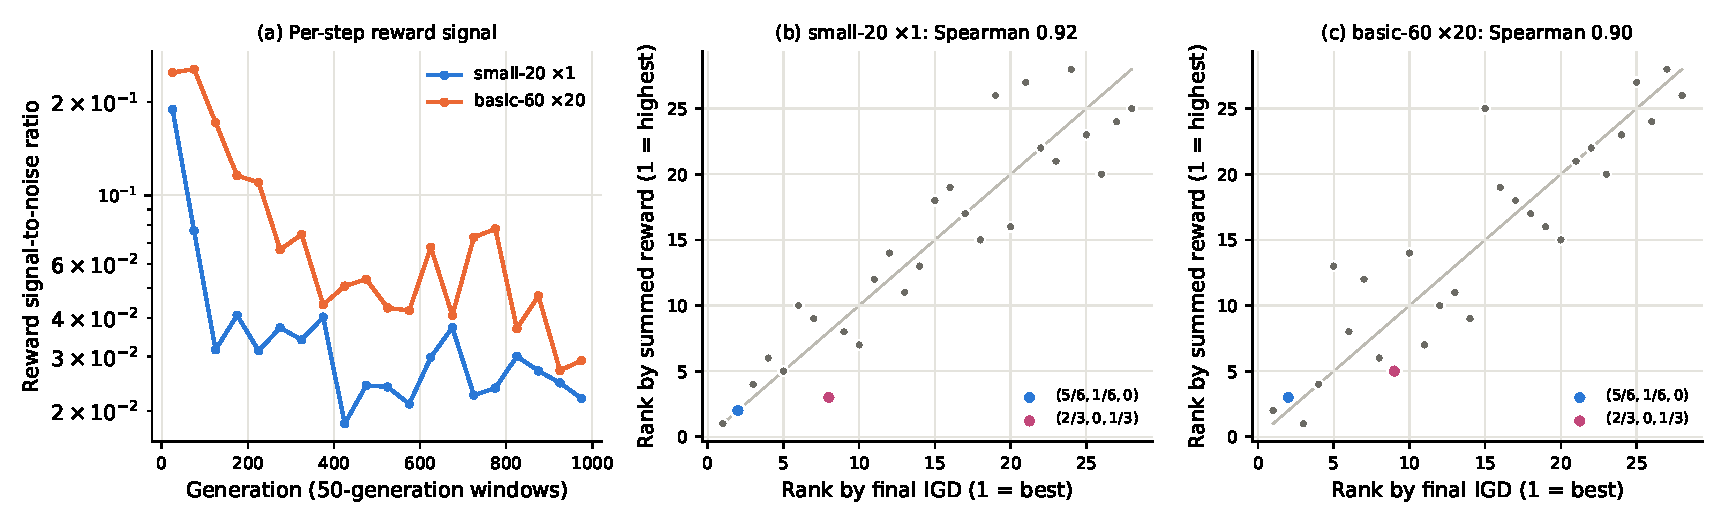
\includegraphics[width=\textwidth]{figures/d1_reward_audit.pdf}
\caption{Reward audit, each of the 28 actions held fixed for 1000 generations. (a) Signal-to-noise ratio of the
per-generation reward. (b, c) Rank of the summed reward against rank by final IGD.}
\label{fig:reward_audit}
\end{figure*}
